\subsection{Utilisation des graphes en génomique comparée}

Les graphes sont largement utilisés en bioinformatique \cite{pavlopoulos_using_2011} et ce dans des domaines très divers : interactions protéine-protéine, expression des gènes, modélisation du métabolisme\dots 

Dans mes travaux de thèse, je me suis largement appuyé sur les méthodes de graphes, il est donc essentiel de revenir sur la terminologie et les concepts liés à la théorie des graphes. Nous utiliserons le graphe de la \autoref{fig:graphe_theorie} pour illustrer les principes suivants.

\begin{figure}[htbp]
    \centering
    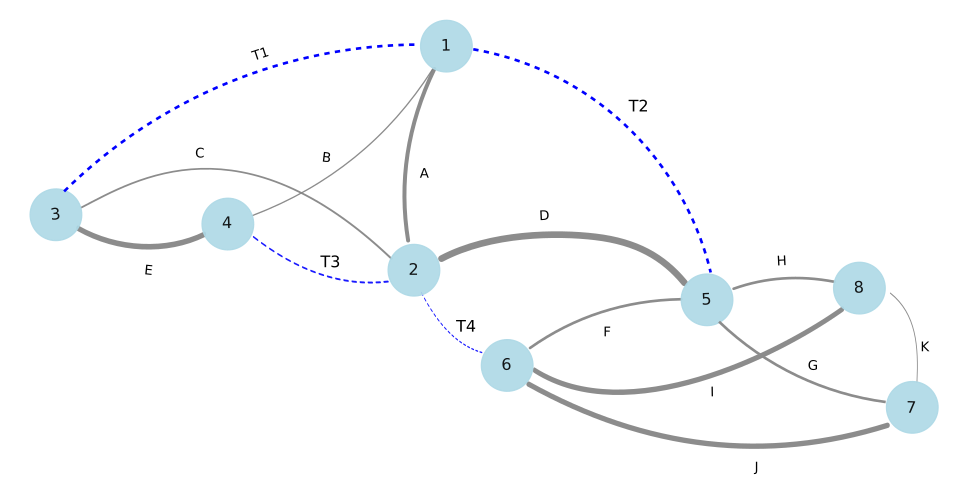
\includegraphics[width=\linewidth]{images/graphe_theorie_non_orienter.png}
    \caption[Exemple de graphe]{\textbf{Exemple de graphe.} Les n\oe uds sont représentés par des cercles et étiquetés par des numéros. Les arêtes, illustrées par des lignes pleines grises et étiquetées par une lettre, définissent les connexions entre les n\oe uds. L’épaisseur des arêtes est proportionnelle à leur poids, indiquant ainsi la valeur associée à chaque connexion. Les arêtes en pointillés bleus représentent les fermetures transitives du graphe, elles sont également étiquetées et pondérées pour expliciter les relations indirectes créées par la transitivité.}
    \label{fig:graphe_theorie}
\end{figure}

\subsubsection{Définitions et concepts}

Un graphe est constitué d'un ensemble de \textbf{n\oe uds} (cercles) reliés par un ensemble d'\textbf{arêtes} (segments gris). Mathématiquement, tous les graphes ne possèdent pas les mêmes propriétés et donc les théorèmes associés changent. Dans la suite, nous utiliserons les symboles mathématiques suivants :
\begin{itemize}
    \item $V$ : ensemble de n\oe uds
    \item $E$ : ensemble d'arêtes
    \item $G(V, E)$ : un graphe composé d'un ensemble de n\oe uds $V$ et d'arête $E$
    \item $u$ et $v$ : 2 n\oe uds distincts dans le graphe
    \item $e_{(u,v)}$ : une arête reliant $u$ et $v$.
\end{itemize}

\paragraph{Orientation du graphe}

Un graphe peut être \textbf{orienté}, \textit{i.e.}, que les arêtes ont une direction. Dans ce cas, il peut exister une arête de $u$ vers $v$ ($e_{(u, v)}$) sans qu'il n'y ait nécessairement une arête $e_{(v, u)}$. Si le graphe est non orienté, si $e_{(u, v)}$ existe, $e_{(v, u)}$ également. Dans notre exemple, le graphe est non orienté.

\paragraph{graphe pondéré et étiqueté}

En bioinformatique, il est courant d'ajouter de l'information sur le graphe. Ces informations peuvent servir à modifier le graphe, le filtrer ou l'analyser, par exemple.

On peut ajouter un \textbf{poids} aux n\oe uds ($w_u$) et aux arêtes ($w_{(u,v)}$), le graphe est alors dit \textbf{pondéré}. Le poids est quantifiable et correspond généralement à un nombre. Dans notre exemple, chaque arête a une épaisseur correspondant à son poids. On peut alors filtrer le graphe pour ne conserver que les arêtes les plus épaisses.

D'autres informations peuvent être ajoutées aux n\oe uds et aux arêtes sous forme d'annotation. Dans ce cas, l'annotation peut être qualitative et on dira que le graphe est \textbf{étiqueté}\footnote{Dans la littérature bioinformatique, on retrouve aussi le terme "coloré", mais qui est utilisé à tort si on se réfère à la théorie des graphes.}. Dans le graphe exemple, les arêtes sont étiquetées par une lettre et les n\oe uds par un chiffre. Cet étiquetage peut notamment correspondre à un identifiant.

\paragraph{Voisinage et chemin dans le graphe}

Dans cette thèse, nous parlerons de n\oe uds \textbf{voisins}, \textit{i.e.}, des n\oe uds qui sont reliés par un ensemble d'arêtes ($E_{(u,v)}$), cet ensemble d'arêtes est appelé \textbf{chemin}. Lorsque $u$ et $v$ sont reliés par une seule arête (chemin de taille 1), on dit qu'ils sont dans un \textbf{voisinage direct}. Dans notre exemple, le n\oe ud 1 est un voisin direct des n\oe uds 2 et 4 et est voisin des n\oe uds 3 et 5 par un chemin de taille 2. Lorsque tous les n\oe uds sont voisins les uns des autres, on dit que le graphe est \textbf{connexe}.

\newpage
\paragraph{Transitivité}

La \textbf{transitivité} dans les graphes est une propriété qui s'applique aux relations entre les n\oe uds. Un graphe est dit \textbf{transitif} si, pour tous n\oe uds $u$, $v$ et $w$, l'existence des arêtes $e_{u,v}$ et $e_{v, w}$, implique qu'il existe $e_{u,w}$. En d'autres termes, si $u$ et $v$ sont reliés et que $v$ et $w$ aussi, alors $u$ et $w$ sont reliés. Dans un graphe orienté transitif, s'il existe $e_{u,v}$ et $e_{v, w}$, alors il existe $e_{u, w}$, mais pas obligatoirement $e_{w, u}$. Cette propriété est particulièrement importante dans les graphes orientés, où elle peut être utilisée pour modéliser des relations hiérarchiques ou des dépendances. 

Dans notre exemple, le graphe n'est pas transitif. Pour le rendre transitif, on ajoute des \textbf{fermetures transitives} entre les n\oe uds. Ces arêtes de transitivité (en pointillés bleus) permettent de compléter le graphe pour le rendre transitif, facilitant ainsi l'analyse des relations et des dépendances implicites entre les n\oe uds.

\paragraph{Sous-ensemble du graphe}

Lorsqu'on va analyser un graphe, on peut chercher à retrouver des structures d'intérêt. Pour commencer, on peut chercher à identifier un \textbf{sous-graphe}. Le sous-graphe est une fraction du graphe qui contient un sous-ensemble de n\oe uds de $G(V, E)$ et les arêtes reliant ces n\oe uds. 

Une autre structure est la \textbf{clique}, qui correspond à un sous-ensemble de n\oe uds tous connectés entre eux. La détection et l'analyse de cliques a de nombreuses applications en bioinformatique, notamment l'identification de groupes de gènes coexprimés. Dans notre exemple, les n\oe uds 5,6,7 et 8 représentent une clique. 

Pour terminer, une forme de sous-ensemble que j'ai largement utilisée, est la \textbf{composante connexe} qui correspond à un ensemble de n\oe uds tel que, quel que soit $u$, $v$, il existe un chemin  qui les relie\footnote{La clique est une composante connexe spéciale où tous les n\oe uds sont reliés par un chemin de taille 1.}.

\paragraph{Partitionnement du graphe}

\textbf{Partitionner} un graphe consiste diviser les n\oe uds du graphe en groupes. Chacun de ces groupes est appelé une \textbf{partie} et l'ensemble des parties est appelé \textbf{partition}. En fonction de l'algorithme utilisé, la partition sera alors différente. Dans ce manuscrit, nous utiliserons cette notion de partition à  de nombreuses reprises.

\subsubsection{Application dans la comparaison des génomes}

L'utilisation des graphes pour la comparaison de génomes est de plus en plus courante. 

Une première application possible est d'améliorer les méthodes de MSA. Des outils comme MUSCLE ou MAFFT \cite{katoh_mafft_2013} utilisent des arbres guides pour améliorer les performances de l'alignement. Ces arbres sont des graphes particuliers, où les séquences sont des n\oe uds et les relations de similarité sont des arêtes.

\newpage
Une seconde utilisation des graphes concerne l'étude des SNPs, indels et SVs. Ces graphes, appelés graphes de variants, représentent d'une manière flexible les différences entre les génomes. Chaque n\oe ud représente une séquence ou un k-mer, les arêtes vont représenter la colocalisation dans le génome. Ainsi, chaque chemin permet de reconstruire un génome, tout en ayant toutes les variations génétiques. Des outils comme VG toolkit \cite{garrison_variation_2018} et Minigraph \cite{li_design_2020}, permettent notamment d'améliorer l'alignement des lectures en sortie de séquençage, mais aussi d'enrichir la représentation des génomes procaryotes présentant une forte diversité.

Une autre application proche des graphes de variants est celle des graphes de réarrangements. Dans ces graphes, les n\oe uds représentent des synténies conservées, les arêtes vont relier ces synténies en fonction de l'ordre et de l'orientation dans les génomes. L'outil Sibelia \cite{minkin_sibelia_2013} est un outil d'alignement et d'analyse des réarrangements de génomes procaryotes. Il permet  d'étudier les différences évolutives et de reconstruire l'histoire des réplicons.

